\begin{figure}[H]
    \centering
    \caption{Representação visual da Diferença Simétrica}
    \label{fig:diferenca_simetrica}
    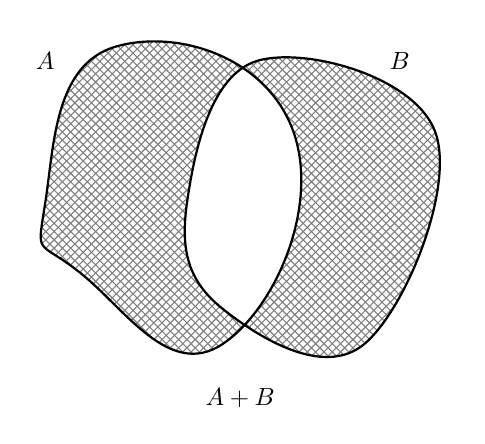
\begin{tikzpicture}[
        scale=0.9,
        transform shape,
        font=\sffamily,
        shaded/.style={
            pattern=crosshatch, 
            pattern color=gray
        }
    ]

    \usetikzlibrary{patterns}

    % Definição das formas
    \def\blobC{plot [smooth cycle, tension=0.9] coordinates {(-2,0) (-1, 2.2) (1.5, 1) (0.5, -2) (-1.5, -1)}}
    \def\blobD{plot [smooth cycle, tension=0.7] coordinates {(0,0) (1, 2) (3.5, 1) (2.5, -2) (0.5, -1.5)}}

    % Diferença Simétrica (A + B)
    \begin{scope}

        \fill[shaded, even odd rule] \blobC \blobD;

        \draw[thick] \blobC;
        \draw[thick] \blobD;

        \node at (-2, 2) {\( A \)};
        \node at (3, 2) {\( B \)};
        \node[below, align=center] at (0.75, -2.5) {\( A + B \)};
    \end{scope}

    \end{tikzpicture}
    \fonte{Elaborado pelo autor (2025).}
\end{figure}